This section presents the \textbf{context view} and the top-level structure of the system. The context view (conforming to the Context viewpoint declared in Section 3) fixes the system boundary and shows the external actors and systems that interact with \productname. The layer descriptions then give the overall structure of the software system --- the strategy for how it will be built.

\begin{figure}[h!]
	\centering
 	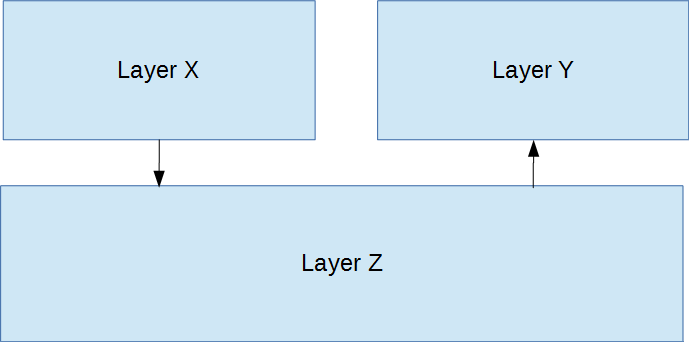
\includegraphics[width=0.60\textwidth]{images/layers}
 \caption{Architectural layer diagram}
\end{figure}

An architectural ``layer'' is the top-level logical view, or abstraction, of your design. Layers should be composed of related elements of similar capability, should be highly independent of other layers, and should have clearly defined interfaces and interactions with other layers. Each layer is identified individually and is unique in its function and purpose within the system. Provide the high-level block diagram of the layers above, and describe the function of each layer below.

\subsection{Layer X Description}
Describe this layer in detail: its features, functions, and the services it provides, and its critical interfaces and interactions with adjacent layers. Note any architecturally significant properties (e.g. this layer is the only one permitted to touch external hardware, or persistent storage).

\subsection{Layer Y Description}
Describe this layer in detail, following the same pattern as Layer X.

\subsection{Layer Z Description}
Describe this layer in detail, following the same pattern as Layer X. Ensure the set of layers is complete (every major responsibility belongs to exactly one layer) and that inter-layer interfaces are consistent with the data-flow view in Section 5.
